\documentclass[aspectratio=169, 8pt, xcolor={svgnames}, hyperref={linkcolor=black}]{beamer}
\usepackage[labelfont={color=amethyst,bf}]{caption}
\setbeamercolor{background canvas}{bg=white}
\usetheme[progressbar=frametitle]{metropolis}
\usepackage{appendixnumberbeamer}
\usepackage{url}
\usepackage{booktabs}
\usepackage{braket}
\usepackage[scale=2]{ccicons}
\usepackage{amsfonts} 
\usepackage{amssymb}
\usepackage[english]{babel}
\colorlet{col1}{teal}
\colorlet{col2}{yellow}
\colorlet{col3}{green}
\usepackage{fontawesome}
\usepackage{amsmath}
\usepackage{subcaption}
\usepackage{multicol}
\usepackage{bm}
\usepackage{algorithm}
\usepackage{overpic}
\usepackage{algpseudocode}
\usepackage{enumitem}

\usepackage[]{pseudo}


\usepackage{tikz}
\usetikzlibrary{positioning,arrows,calc,math,angles,quotes}
\usepackage{blochsphere}


\usetikzlibrary{arrows,automata}
\usetikzlibrary{positioning}
\usetikzlibrary{arrows.meta,
                bending,
                intersections,
                quotes,
                shapes.geometric}

\tikzset{
    state/.style={
           rectangle,
           rounded corners,
           draw=black, very thick,
           minimum height=1em,
           inner sep=2pt,
           text centered,
           },
}


\definecolor{myv}{rgb}{0.36, 0.22, 0.33}
\definecolor{gio}{rgb}{0.45, 0.31, 0.59}
\definecolor{light}{rgb}{0.8, 0.8, 1}
\definecolor{warmblack}{rgb}{0.0, 0.26, 0.26}
\definecolor{brown(web)}{rgb}{0.65, 0.16, 0.16}
\definecolor{cadmiumgreen}{rgb}{0.0, 0.42, 0.24}
\definecolor{darkmidnightblue}{rgb}{0.0, 0.2, 0.4}
\definecolor{brightube}{rgb}{0.82, 0.62, 0.91}
\definecolor{carnelian}{rgb}{0.7, 0.11, 0.11}
\definecolor{codegreen}{rgb}{0,0.6,0}
\definecolor{codegray}{rgb}{0.5,0.5,0.5}
\definecolor{codepurple}{rgb}{0.58,0,0.82}
\definecolor{backcolour}{rgb}{0.95,0.95,0.92}
\definecolor{amethyst}{rgb}{0.6, 0.33, 0.73}

\definecolor{light-gray}{gray}{0.95}
\newcommand{\code}[1]{\colorbox{light-gray}{\texttt{#1}}}


\usepackage{listings}
\lstdefinestyle{mystyle}{
    backgroundcolor=\color{backcolour},   
    commentstyle=\color{codegreen},
    keywordstyle=\color{codepurple},
    numberstyle=\tiny\color{codepurple},
    stringstyle=\color{magenta},
    basicstyle=\footnotesize,
    breakatwhitespace=false,         
    breaklines=true,                 
    captionpos=b,                    
    keepspaces=true,                 
    numbers=left,                    
    numbersep=5pt,                  
    showspaces=false,                
    showstringspaces=false,
    showtabs=false,                  
    tabsize=2
}

\lstset{style=mystyle}
\usepackage[most]{tcolorbox}
\usepackage{xcolor}


%\usepackage[citecolor = green, linkcolor = blue, bookmarks=true, urlcolor=blue,
%colorlinks=true, pagebackref=true]{hyperref}


%\usepackage{xspace}

\title{Quantum Noise and error mitigation}
\subtitle{Quantum Computing Minicourse ICTP-SAIFR}
\date{8 April 2024}
\author{Stefano Carrazza$^\ddag$ and Matteo Robbiati$^\dagger$}
\institute{$^\ddag$ Associate Professor \& Researcher, University of Milan and INFN Milan, Italy.\\
$^\dagger$ PhD candidate, University of Milan, Italy and CERN, Switzerland.}

\begin{document}

\begin{frame}
\maketitle
\begin{picture}(0,0)
    \put(270,40){
        
\includegraphics[width=0.25\textwidth]{figures/qibo_noise.png}
    }
\end{picture}
\end{frame}

\begin{frame}{Various sources of noise}
We call \textbf{quantum noise} any phenomenon that can corrupt the 
manipulation of the state of a system of qubits. \pause

We can introduce various sources of noise.
\begin{figure}
    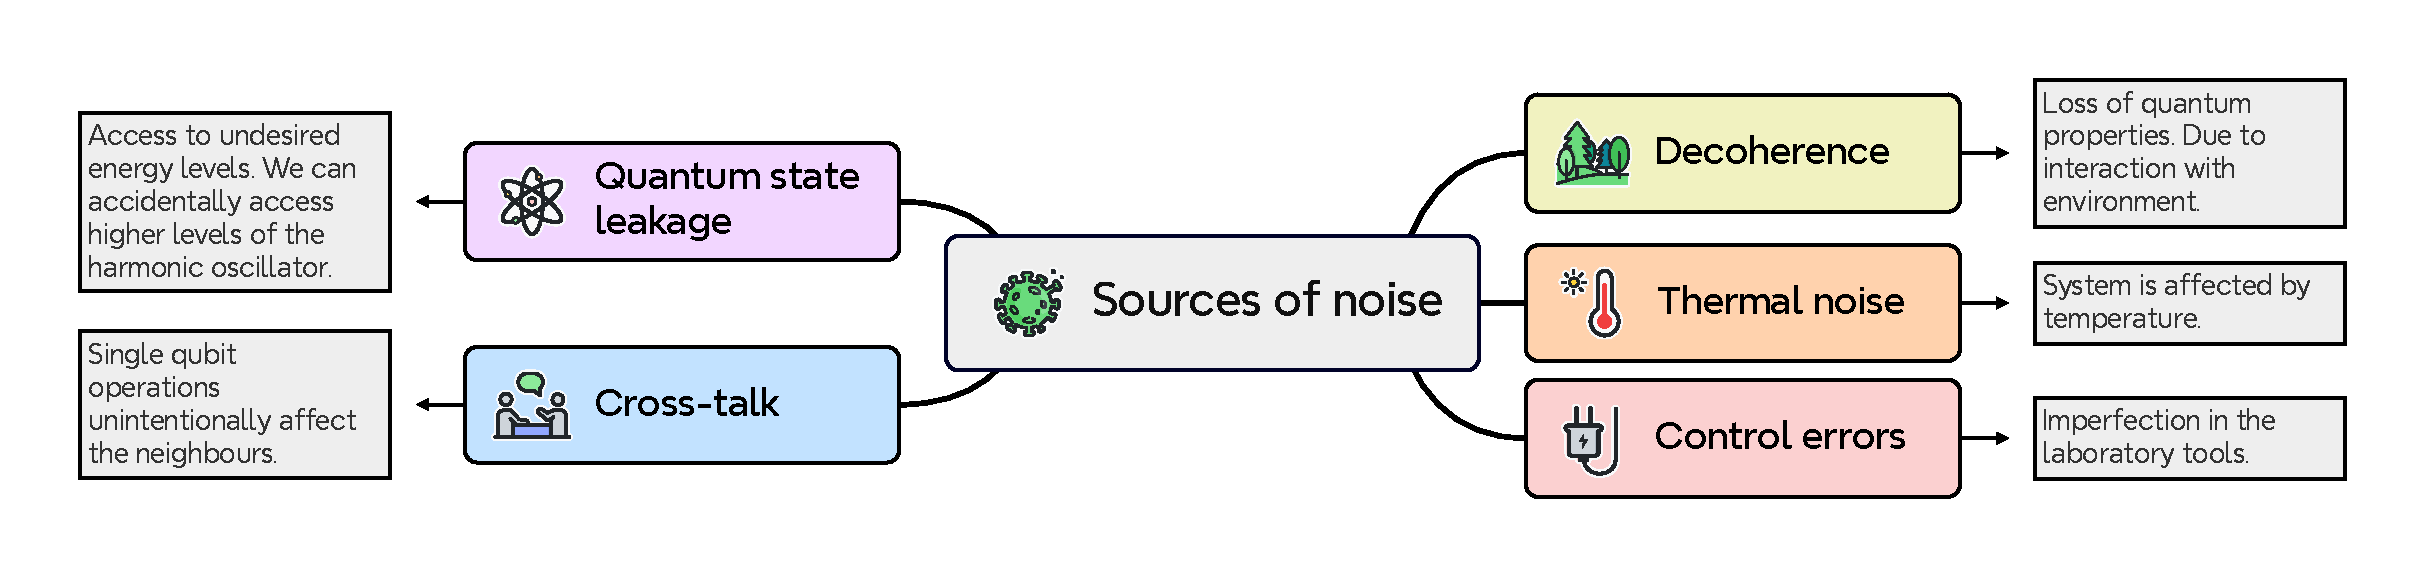
\includegraphics[width=1\textwidth]{figures/noises.pdf}
\end{figure}
\pause
Each of them (even all together) can deteriorate a quantum state.

\pause
\textcolor{carnelian}{What about the shot-noise? Is it similar to these noises?}
\end{frame}

\begin{frame}{Without noise we can use state vectors}

For now we talked about state vector manipulation, where unitary 
gates $\mathcal{U}$ are used to evolve quantum states:
$$ \ket{\psi}' = \mathcal{U} \ket{\psi}. $$ \pause
This picture is fine until the quantum state is \textbf{pure}, namely, it is 
represented by a vector into the Hilbert space. \pause

\begin{multicols}{2}
\texttt{\\}
\textbf{About pure states}

{\footnotesize\faCircle\,\,}Pure states are preserved until the quantum system is isolated, thus
doesn't interact with the environment. 

{\footnotesize\faCircle\,\,}A pure state of a single qubit can be visualized as a point on the surface
of the Bloch sphere. 

{\footnotesize\faCircle\,\,}Using unitaries $\mathcal{U}$ we can move any point of the sphere into 
another point in a reversible way. 
\begin{center}
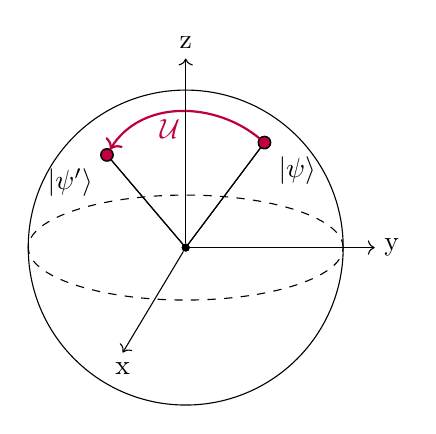
\begin{tikzpicture}

  % Define radius
  \def\r{2}

  \draw (0, 0) node[circle, fill, inner sep=1] (orig) {} -- (\r/2, \r/1.5) node[circle, fill, inner sep=0.7,minimum size=5pt] (a) {};
  \draw (0, 0) node[circle, fill, inner sep=1] (orig) {} -- (\r/2, \r/1.5) node[circle, fill=purple, inner sep=0.7, minimum size=4pt, label=below right:$\ket{\psi}$] (a) {};

  % Bloch vector
  \draw (0, 0) node[circle, fill, inner sep=1] (orig) {} -- (-\r/2, \r/1.7) node[circle, fill, inner sep=0.9,minimum size=5pt] (aprime) {};
  \draw (0, 0) node[circle, fill, inner sep=1] (orig) {} -- (-\r/2, \r/1.7) node[circle, fill=purple, inner sep=0.9, minimum size=4pt, label=below left:$\ket{\psi'}$] (aprime) {};

  \draw[purple, thick, ->] (a) to[out=140, in=60] (aprime);
  \node[purple] at (-0.2,1.5) {$\mathcal{U}$};

  % Sphere
  \draw (orig) circle (\r);
  \draw[dashed] (orig) ellipse (\r{} and \r/3);

  % Axes
  \draw[->] (orig) -- ++(-2*\r/5, -2*\r/3) node[below] (x1) {x};
  \draw[->] (orig) -- ++(1.2*\r, 0) node[right] (x2) {y};
  \draw[->] (orig) -- ++(0, 1.2*\r) node[above] (x3) {z};

\end{tikzpicture}
\end{center}

\end{multicols}

\end{frame}

\begin{frame}{The noise breaks the vector notation!}
\textcolor{carnelian}{But what happens if we have noise?} \pause State vectors 
are no longer usable, because the system is not isolated. \pause

Noise corrupts the quantum states, building \textbf{mixed states}, namely classical 
mixture of pure states. \pause An useful tool to represent both pure and mixed states is the \textbf{density matrix}, 
which in general is defined as:
$$ \rho = \sum_{i=0}^n p_i \ket{\psi_i}\bra{\psi_i}, $$
where $p_i$ is the statistical weight of the pure state $\ket{\psi_i}$ in the mix. 
If $n=1$, then $\rho=\ket{\psi}\bra{\psi}$ and $\ket{\psi}$ is pure. \pause

\begin{multicols}{2}
\textbf{About mixed states}

{\footnotesize\faCircle\,\,} The evolution of a density matrix is described in terms 
of superoperators $\rho' = \mathcal{E} (\rho)$, which, in the case of pure states 
act like unitaries $ \rho' = \mathcal{E}^{\dagger} \rho \mathcal{E}. $ 

{\footnotesize\faCircle\,\,} A mixed state of a single qubit can be visualized as a point within the surface
of the Bloch sphere. 

{\footnotesize\faCircle\,\,} The effect of the noise can be represented by a superoperator
which can map points on the surface into points located within the Bloch sphere.     
\begin{center}
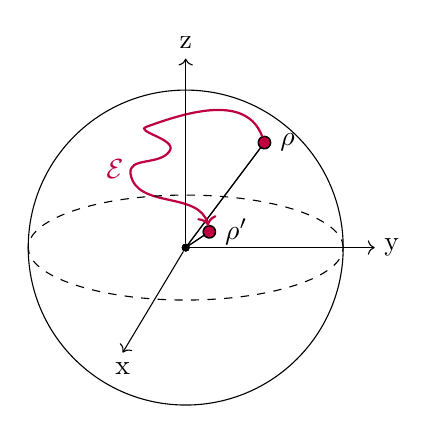
\begin{tikzpicture}

  % Define radius
  \def\r{2}

  \draw (0, 0) node[circle, fill, inner sep=1] (orig) {} -- (\r/2, \r/1.5) node[circle, fill, inner sep=0.7,minimum size=5pt] (a) {};
  \draw (0, 0) node[circle, fill, inner sep=1] (orig) {} -- (\r/2, \r/1.5) node[circle, fill=purple, inner sep=0.7, minimum size=4pt, label=right:$\rho$] (a) {};

  % Bloch vector
  \draw (0, 0) node[circle, fill, inner sep=1] (orig) {} -- (0.3*\r/2, 0.3*\r/3) node[circle, fill, inner sep=0.7,minimum size=5pt] (aprime) {};
  \draw (0, 0) node[circle, fill, inner sep=1] (orig) {} -- (0.3*\r/2, 0.3*\r/3) node[circle, fill=purple, inner sep=0.7, minimum size=4pt, label=right:$\rho'$] (aprime) {};

  \draw[purple, thick, ->] (a) to[out=110, in=20] ++(-1.5,0.2) to[out=200, in=60] ++(0.3,-0.3) to[out=240, in=100] ++(-0.5,-0.3) to[out=280, in=100] (aprime);
  \node[purple] at (-0.9,1) {$\mathcal{E}$};

  % Sphere
  \draw (orig) circle (\r);
  \draw[dashed] (orig) ellipse (\r{} and \r/3);

  % Axes
  \draw[->] (orig) -- ++(-2*\r/5, -2*\r/3) node[below] (x1) {x};
  \draw[->] (orig) -- ++(1.2*\r, 0) node[right] (x2) {y};
  \draw[->] (orig) -- ++(0, 1.2*\r) node[above] (x3) {z};

\end{tikzpicture}
\end{center}
\end{multicols}

\end{frame}

\begin{frame}{Pure and mixed states in the Bloch sphere}
\pause
\small
\begin{multicols}{2}
\textbf{The maximally entangled state is a pure state}

The density matrix of $\ket{+} = \frac{1}{\sqrt{2}}(\ket{0}+\ket{1})$ is 
\begin{multline*}
$$\rho_{\rm pure} = \ket{+}\bra{+} =
\\ = \begin{bmatrix} 1/\sqrt{2} & 1/\sqrt{2}  \end{bmatrix}\begin{bmatrix} 
1/\sqrt{2} \\ 1/\sqrt{2} \end{bmatrix} = \begin{bmatrix} 1/2 & 1/2 \\ 1/2 & 1/2  \end{bmatrix} $$
\end{multline*}
\begin{center}
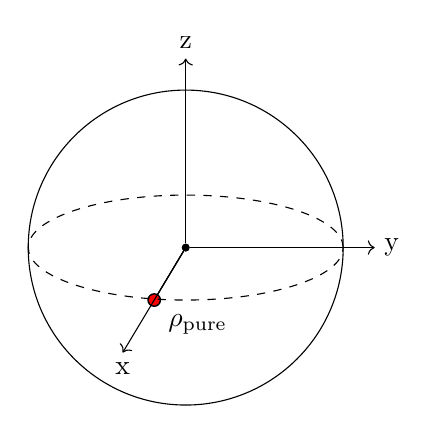
\begin{tikzpicture}

  % Define radius
  \def\r{2}

  % Bloch vector
  \draw (0, 0) node[circle, fill, inner sep=1] (orig) {} -- (-\r/5, -\r/3) node[circle, fill, inner sep=0.7,minimum size=5pt] (a) {};
  \draw (0, 0) node[circle, fill, inner sep=1] (orig) {} -- (-\r/5, -\r/3) node[circle, fill=red, inner sep=0.7, minimum size=4pt, label=below right:$\rho_{\rm pure}$] (a) {};

  % Sphere
  \draw (orig) circle (\r);
  \draw[dashed] (orig) ellipse (\r{} and \r/3);

  % Axes
  \draw[->] (orig) -- ++(-2*\r/5, -2*\r/3) node[below] (x1) {x};
  \draw[->] (orig) -- ++(1.2*\r, 0) node[right] (x2) {y};
  \draw[->] (orig) -- ++(0, 1.2*\r) node[above] (x3) {z};

\end{tikzpicture}
\end{center}

\textbf{The state which maximally mix $\ket{0}$ and $\ket{1}$}

The density matrix of $\frac{1}{2} \bigl( \ket{0}\bra{0} + \ket{1}\bra{1} \bigr)$ is
\begin{multline*}
\rho_{\rm mix} = \frac{1}{2} \bigl( \ket{0}\bra{0} + \ket{1}\bra{1} \bigr) =
\\\frac{1}{2} \begin{bmatrix} 1 & 0  \end{bmatrix}\begin{bmatrix} 
1 \\ 0\end{bmatrix} + \frac{1}{2} \begin{bmatrix} 0 & 1  \end{bmatrix}\begin{bmatrix} 
0 \\ 1\end{bmatrix} = \begin{bmatrix} 1/2 & 0 \\ 0 & 1/2  \end{bmatrix} 
\end{multline*}
\begin{center}
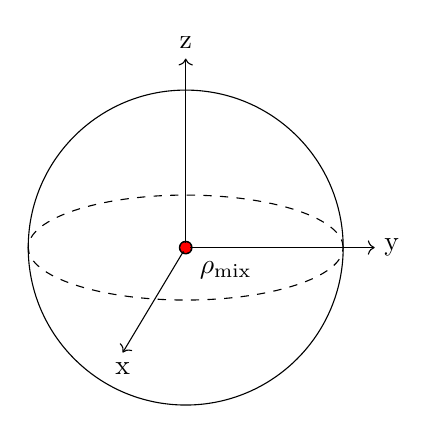
\begin{tikzpicture}

  % Define radius
  \def\r{2}

  % Bloch vector
  \draw (0, 0) node[circle, fill, inner sep=1] (orig) {} -- (0, 0) node[circle, fill, inner sep=0.7,minimum size=5pt] (a) {};
  \draw (0, 0) node[circle, fill, inner sep=1] (orig) {} -- (0, 0) node[circle, fill=red, inner sep=0.7, minimum size=4pt, label=below right:$\rho_{\rm mix}$] (a) {};

  % Sphere
  \draw (orig) circle (\r);
  \draw[dashed] (orig) ellipse (\r{} and \r/3);

  % Axes
  \draw[->] (orig) -- ++(-2*\r/5, -2*\r/3) node[below] (x1) {x};
  \draw[->] (orig) -- ++(1.2*\r, 0) node[right] (x2) {y};
  \draw[->] (orig) -- ++(0, 1.2*\r) node[above] (x3) {z};

\end{tikzpicture}
\end{center}
\end{multicols}
\end{frame}

\begin{frame}{The Pauli representation of the noise}
We can now define a superoperator $\mathcal{N}$, which represents the action of the 
noise on a state:
$ \rho_{\rm noisy} = \mathcal{N}(\rho). $ \pause

We can exploit the Pauli's operator to write a noise model:
\begin{itemize}[noitemsep]
\item[-] we use $X$ to apply random bitflip $\ket{0}=X\ket{1}$ and $\ket{1}=X\ket{0}$ with probability $p_x$;
\item[-] we use $Z$ to apply random phase flip $\ket{0}=Z\ket{0}$ and $-\ket{1}=Z\ket{1}$ with probability $p_z$;
\item[-] we use $Y$ to apply more complex manipulations since $Y=iXZ$ with probability $p_y$. \pause
\end{itemize}
Then the combined effect of these Pauli components is:
$$ \mathcal{N}(\rho) = \textcolor{purple}{\biggl(1 - \sum_{k}p_k\biggr) \rho} + \sum_k p_k P_k \rho P_k $$
where $\sum_k p_k \leq 1$, $P_k$ are the Paulis $\{X, Y, Z\}$
 and the \textcolor{purple}{first term} describe when $\rho$ remains unchanged. \pause

\vspace{0.2cm}
\begin{tcolorbox}[colback=red!15, title=Effect of the noise when computing expectation values]
\begin{itemize}[noitemsep]
\item[1.] The effect of this noise model is to push any state $\rho$ closer to the maximally mixed state $\rho_{\rm mix}=\frac{1}{2^N} I$, 
where $N$ is the number of qubits of the system.
\item[2.] The expectation value of a Pauli observable ($X, Y, Z$ or a combination $P$) over $\rho_{\rm mix}$ is zero.
\item[3.] From 1. and 2., the more intense is the noise, the more $\braket{\rho|P|\rho}\to 0$
\end{itemize}
\end{tcolorbox}

\end{frame}

\begin{frame}{How can we face this problem?}
\begin{figure}
    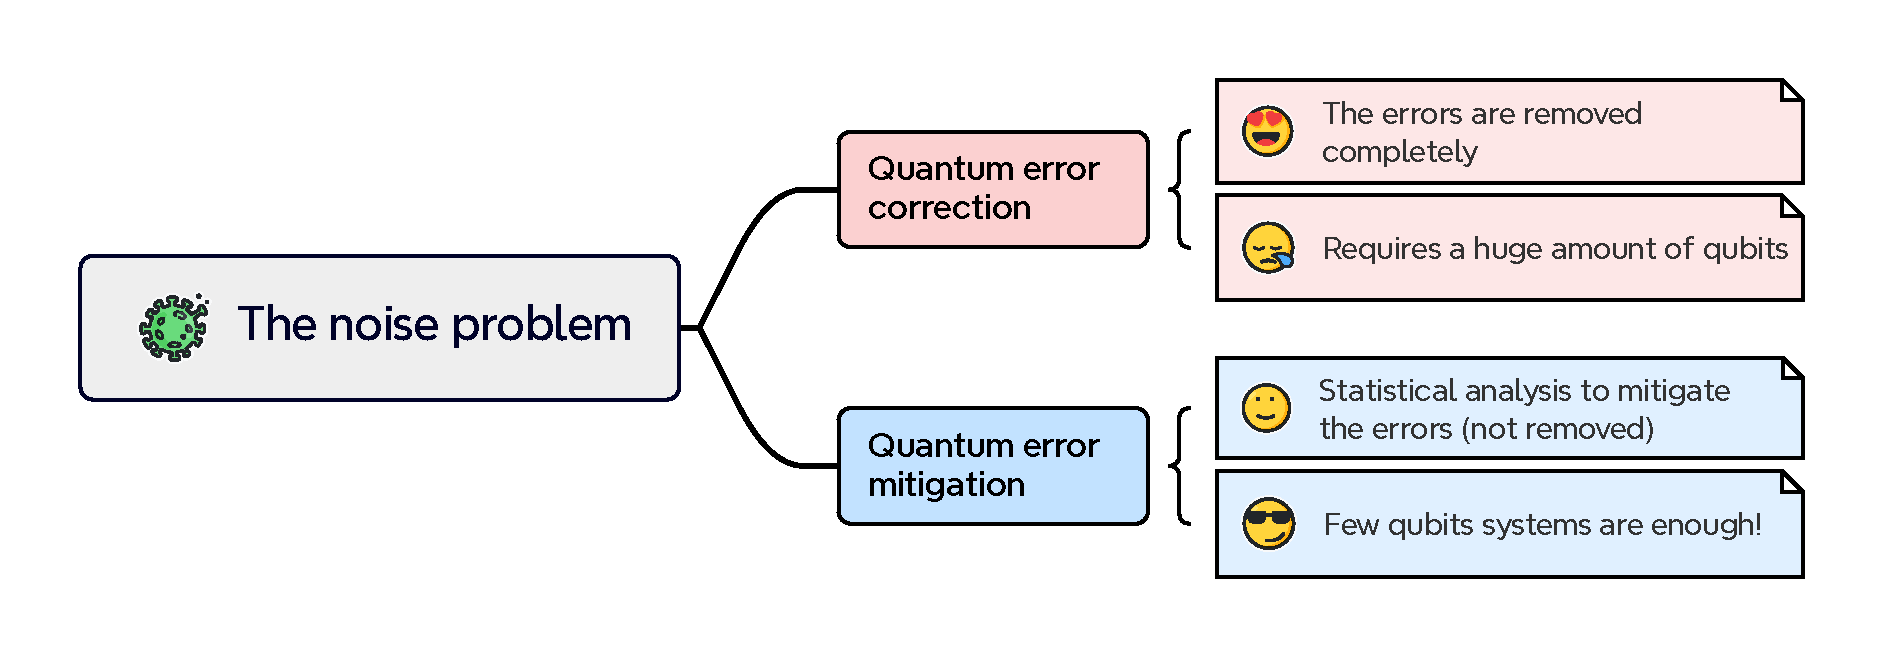
\includegraphics[width=1\textwidth]{figures/qem_qec.pdf}
\end{figure}
\end{frame}

\begin{frame}{Clifford Data Regression}
\textcolor{carnelian}{The goal of quantum error mitigation is to use our knowledge about 
the noise to try to mitigate its effect.} \pause

Suppose we are interested in computing the expectation value $\braket{\mathcal{O}}^0$ 
of an observable $\mathcal{O}$
over the state we get applying the quantum circuit $\mathcal{C}^0$ to a state $\rho$. \pause

But our system is noisy! Thus what we get is a noisy expectation value $\braket{\mathcal{O}}^0_{\rm noisy}$. \pause

\begin{multicols}{2}
\textbf{Clifford Data Regression algorithm}
\begin{itemize}[noitemsep]
\item[1.] We sample a set of circuits $\mathcal{C}^i_{\rm cdr}$, of the 
same size of the target $\mathcal{C}^0$, but which are fast simulable.
\item[2.] For each of these $C^i_{\rm cdr}$ we calculate both exact and 
noisy expectation value.
\item[3.] Make a scatter plot of exact versus noisy expectation values and fit 
the points with a line.
\item[4.] This line is actually a noise map, which can be used to map our $\mathcal{C}^0_{\rm noisy}$
into $\mathcal{C}^0$.
\item[5.] The obtained map can be used for any new circuit of the same size of $\mathcal{C}^0$.
\end{itemize}
\begin{figure}
    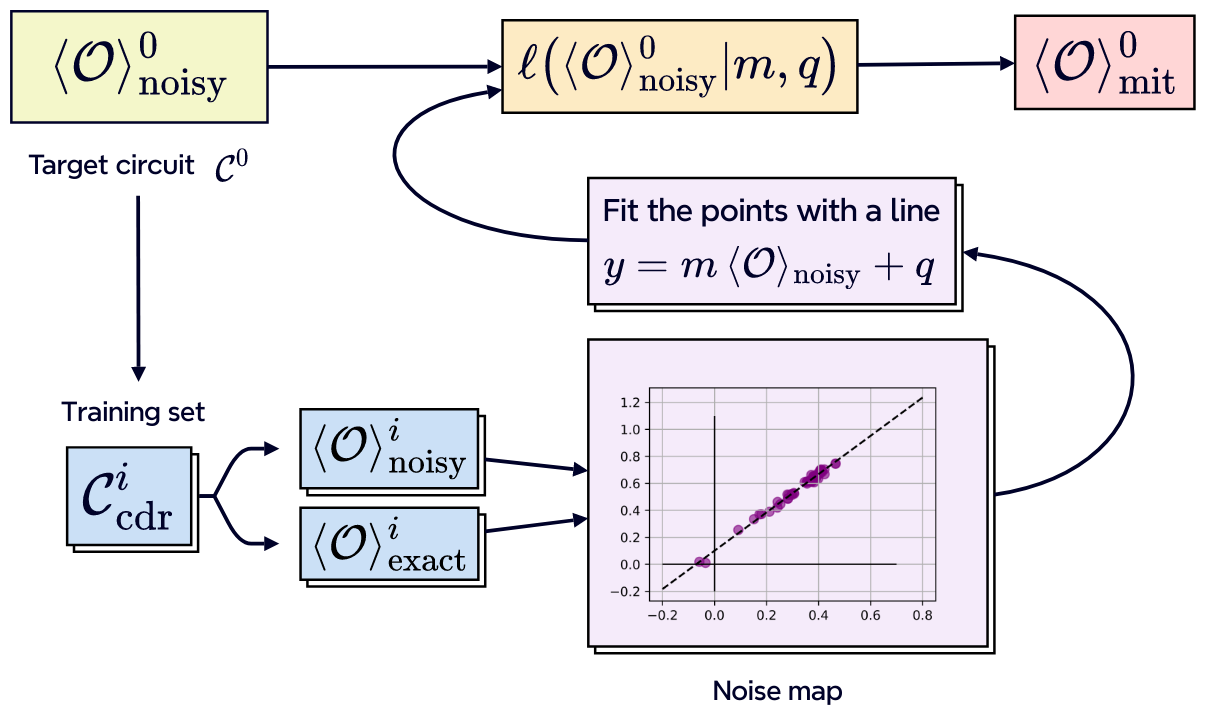
\includegraphics[width=0.5\textwidth]{figures/cdr.png}
\end{figure}
\end{multicols}

\end{frame}

\begin{frame}
\centering
\Huge Let's code!
\begin{figure}
   
\includegraphics[width=0.7\textwidth]{figures/hands_on.png}
\end{figure}
\end{frame}

\end{document}
